%%% Clinic Statement of Work Template
%%%
%%% C.M. Connelly <cmc@math.hmc.edu>
%%%
%%%  $Id: statement-of-work-template.tex 353 2010-08-23 23:47:44Z cmc $


%%% !!! HMC STUDENTS SHOULD REMOVE THE FOLLOWING COPYRIGHT NOTICE FROM
%%% !!! FINAL SUBMISSIONS.

%%% Copyright (C) 2004-2010 Department of Mathematics, Harvey Mudd College.
%%%
%%% This file is part of the hmcclinic class document provided to
%%% HMC mathematics students.
%%%
%%% See the COPYING document, which should accompany this
%%% distribution, for information about distribution and
%%% modification of the document and its components.

%%% !!! END COPYRIGHT NOTICE.


%%% Clinic reports use the clinic class, which should be located
%%% somewhere in TeX's search path.

%%% For your ``statement of work'' (or ``work statement''), specify
%%% the ``proposal'' document-class option to the hmcclinic class.
\documentclass{hmcclinic}
\usepackage{graphicx}

%%% The major difference between the statement of work and a midyear
%%% or final report is that the statement of work is typeset as an
%%% article, which means that the highest level of structural
%%% division available to you is section rather than chapter.

%%% There are also some changes in pagination styles and content
%%% that reflect the briefer nature of the proposal.  For example,
%%% in the longer reports, you use \frontmatter, \mainmatter, and
%%% \backmatter to separate some sections of the report from
%%% others.  In the statement of work, you don't need those
%%% commands, as no such division is necessary.

%%% Other packages needed by your document may be loaded here.
% \usepackage{url}              % For formatting URLs and other web or
                                % file references.

%%% Provide additional context around errors. 
\setcounter{errorcontextlines}{1000}


%%% Information about this document.

%%% I find it most useful to put identifying information about a
%%% document near the top of the preamble.  Technically, this
%%% information must precede the \maketitle command, which often
%%% appears immediately after the beginning of the document 
%%% environment.  Placing it near the top of the document makes it
%%% easier to identify the document, and keeps it out from getting
%%% mixed up with the real meat of the document.

%%% We use the same set of commands for specifying information about
%%% the people involved with the project that are used in the longer
%%% reports, so you can copy most of this information directly into
%%% your midyear and final reports.

%%% So, some questions.

%% What is the name of the company or organization sponsoring your project?
\sponsor{SpaceX}

%% What is the title of your report?
\title{Process Time Analysis In Spaceflight}

%% Who are the authors of the report (your team members)?  (Separate
%% names with \and.)
\author{Wendy Brooks~(Fall Project Manager) \and May Lynn Forssen~(Spring Project Manager) \and Alix Joe \and
Rachel Macfarlane}

%% What is your faculty advisor's name?  (Again, separate names with
%% \and, if necessary.)
\advisor{Ben Wiedermann}

%% Liaison's name or names?
\liaison{Jesse Keller \and Jessica Hester \and Jim Gruen}

%%% End of information section.

%%% New commands and environments.

%%% You can define your own commands and environments here.  If you
%%% have a lot of material here, you might want to consider splitting
%%% the commands and environments into a separate ``style'' file that
%%% you load with \usepackage.

\newcommand{\coolcommand}[1]{#1 is cool.} % Lets everyone know that
                                % the person or thing that you provide
                                % as the argument to the command is
                                % cool.


%%% Some theorem-like command definitions.

%%% The \newtheorem command comes from the amsthm package.  That
%%% package is loaded by the class file.

%%% Note that these definitions have changed from the version in the
%%% sample report document by dropping the ``within'' argument.  See
%%% Gratzer's _Math into LaTeX_ or the AMS-LaTeX documentation for
%%% more details.

% \newtheorem{thm}{Theorem}
% \newtheorem{Theo1}{Theorem}
% \newtheorem{Theo2}{Theorem}
% \newtheorem{Lemma}{Lemma}


%%% If you find that some words in your document are being hyphenated
%%% incorrectly, you can specify the correct hyphenation using the
%%% \hyphenation command.  Note that words are separated by
%%% whitespace, as shown below.

\hyphenation{ap-pen-dix wer-ther-i-an}


%%% The start of the document!

%% The document environment is the main environment in any LaTeX
%% document.  It contains other environments, as well as your text.

\usepackage{float}
\restylefloat{table}
\begin{document}

%%% In a longer document (such as your midterm and final reports),
%%% you would have separate \frontmatter, \mainmatter, and
%%% \backmatter commands to define some large chunks of your
%%% document.  For the Statement of Work, which is a short document,
%%% we don't need these commands.

%%% Your Statement of Work begins with a title page.  The title page
%%% is formatted by commands in the document class file, so you
%%% don't need to worry about what it looks like -- just putting the
%%% \maketitle command in your document (and filling in the necessary
%%% information for the identification commands above) is enough.
\maketitle

%%% In a longer document or an article being submitted to a journal
%%% or conference, you would probably have an abstract that
%%% summarized the purpose of the document.  We don't need that for
%%% a Statement of Work.

%%% Similarly, in longer documents you would probably have commands
%%% to include a table of contents and lists of figures or tables.
%%% For a short document such as the Statement of Work, we don't
%%% need these commands.


%%% Content.
\chapter{Background} % May Lynn
\section{Introduction}
SpaceX is an American space transport company that designs and manufactures
advanced rockets and spacecrafts. The eventual goal of the company is to allow
people to live on other planets. SpaceX rockets depend on a variety of software
to be successful, including simulations, flight software, and data analysis.
Almost all of this software is written in-house and is complex enough that subtle
problems are often hard to catch and very time consuming to debug.

%\section{Background} % May Lynn
\section{Tracing and Debugging}
The data that SpaceX developers examine in order to find software bugs is called
a kernel trace, which documents the different tasks running on a computer over a
certain span of time, keeping track of when each task was running on each processor. 

% Several computers are on board each SpaceX rocket and rely on tasks running in
% predictable, cyclical patterns to coordinate. An unexpected preemption, priority
% inversion, or some break in the pattern of tasks being run can cause problems
% for the rocket.
In order to find potential bugs in their software, SpaceX developers look for
problems like unexpected preemptions, priority inversions, and breaks in the
pattern of tasks being run. A preemption occurs when one program is running, and
is then blocked by another program starting to run on the same CPU. A priority
inversion occurs when a high-priority task is indirectly blocked by something of
lower priority using up a shared resource that the higher priority task needs in
order to run. The software running on SpaceX rockets has deadlines for tasks at regular intervals because timing is very important in rocket flight, so when there is a break in this cyclical pattern of processes this means that there is likely a bug in the software.
\section{Existing Tool}
SpaceX currently uses a tool called kernelshark to visualize this trace data and help find any bugs or anomalies. We were informed by our liaisons that this debugging process can take up to several days, so searching for bugs using this tool uses up a lot of valuable time. Much of the user expeience of kernelshark is outdated or could use improvements. The kernelshark tool consists of a graphical display of the programs running on a computer over time, as well as a tabular view of the same information, in the form of CPU events such as processes switching, waking, or sleeping.
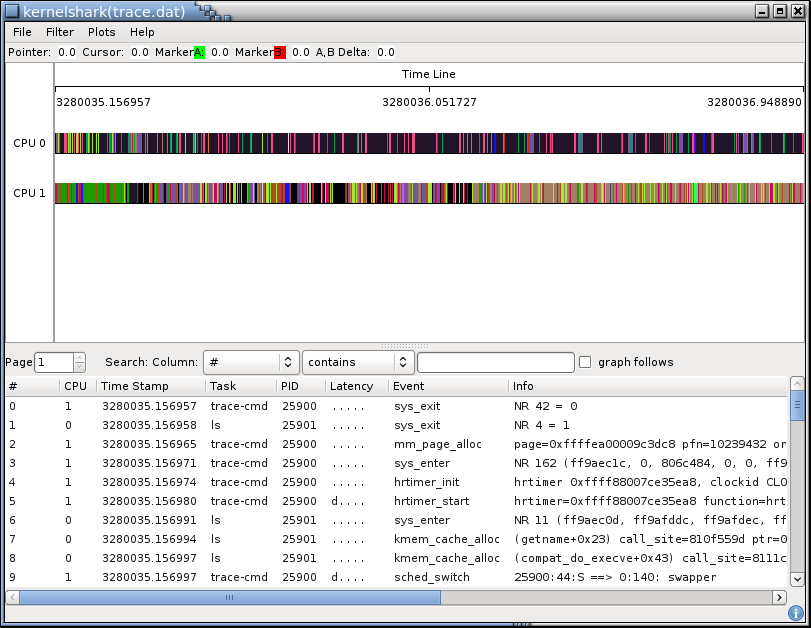
\includegraphics[width=5in]{kshark-open.png}\\
\\
Using only this visualization, it can be difficult to see where the cyclical
deadlines for the programs begin and end, making it hard to find when something
misses a deadline. In addition, the tabular display of the CPU events in the
bottom part of the screen has minimal search functionality and the different
columns of the table are not sortable. Individual timelines for tasks can be
displayed below this main chart, but the menu to select a task does not have
any searching capability and does not order the tasks in any discernable way.

\section{Project Goals} % May Lynn
Our goals for this project were to make it easier and faster for SpaceX engineers to find software problems by creating a tool that visualizes rocket data and highlights problem areas. We have created an improved user experience and provided more visualizations of the data than the old tool. We have called the tool that we created SpaceShark.

\chapter{SpaceShark}
\section{Design} %Everyone gets a part

  SpaceShark is meant to make it easier for SpaceX engineers to find bugs. We
  accomplish this through a variety of pages that serve unique purposes, giving
  engineers many options in how they want to approach finding a problem. First
  we describe briefly the method we used to make the pages, and then describe
  the purpose of each page in the tool and how they accomplish their
  respective goals.

  \subsection{Nodewebkit and HTML} %Rachel
    At the beginning of the project, the team researched possible tools and
    technologies for creating our application. One possibility was simply
    extending kernelshark, the existing tool. After looking at the code for
    this, a large number of C files, we decided it would be easier to
    reimplement and extend it in something else; understanding the code base
    would take a very long time, and we felt other languages had better
    UI and charting libraries. We looked into Java UI libraries for
    desktop applications, as well as web-technology based charting libraries.
    During this research, we found node-webkit, which allows for
    HTML/CSS/Javascript applications to be packaged and run as desktop
    applications with no reliance on the internet. As this allowed us to take
    advantage of many existing UI widgit and charting libraries that many team
    members were familar with, we decided to take this route.

\subsection{Load File Page}
\begin{center}
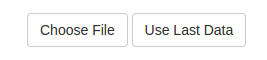
\includegraphics[scale=0.75]{loadFile-buttons.png}
\end{center}
The purpose of the Load file page is to allow the user to choose which JSON file to load as their data, or choose to use the data that was previously used if this is not the user's first time using the tool. This allows the user to easily resume their work if they were previously examining a specific file.

The code for the Load File page can be found in assets/js/loadFile.js.
  \subsection{Overview Page} 
  
  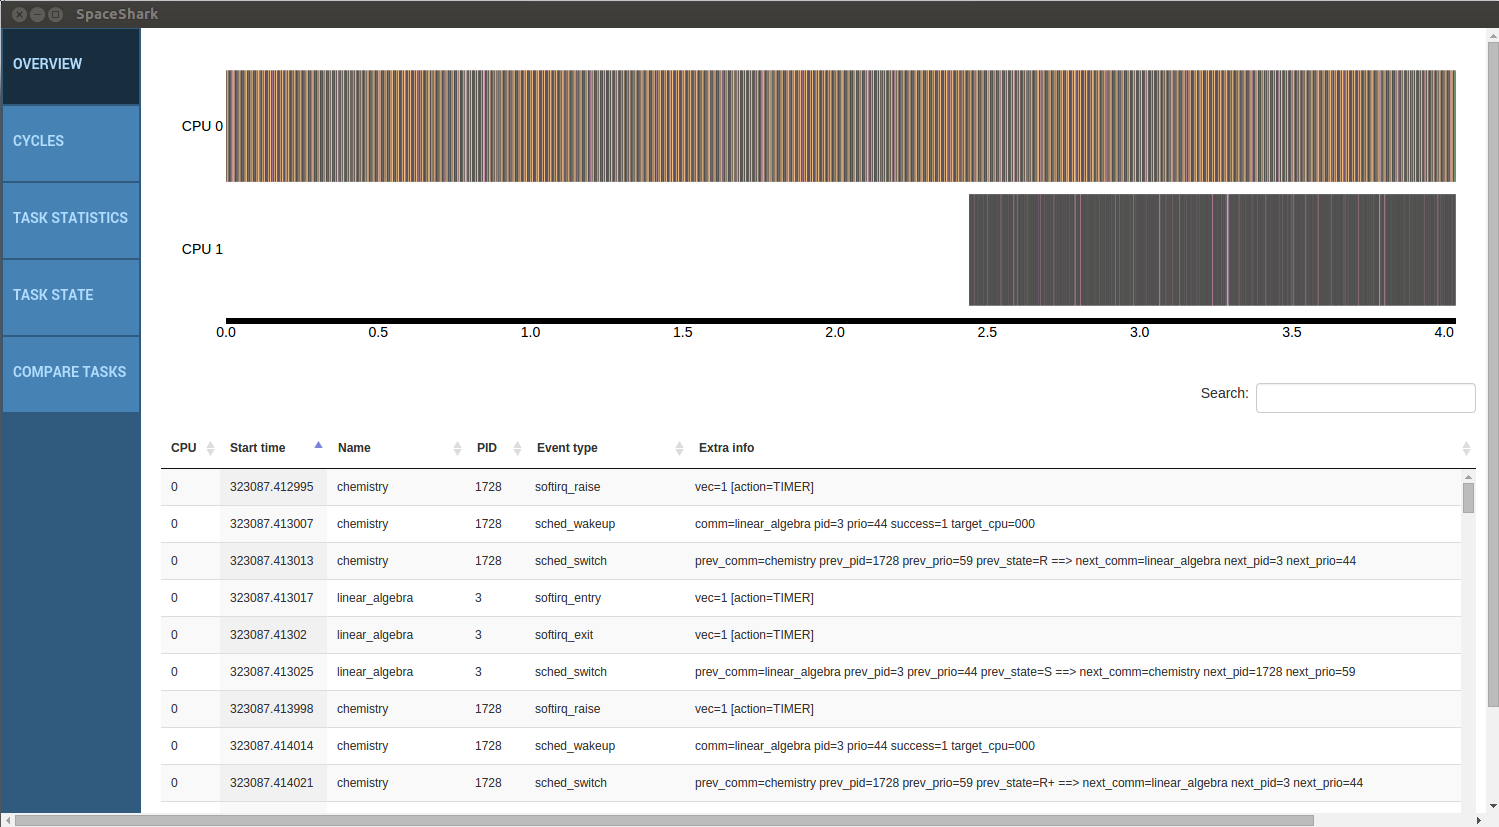
\includegraphics[scale=0.25]{overview-page.png}
  
The purpose of the Overview Page is to be able to look at an overview of all the data, and then later be able to look at more specific details that are of particular interest to the user.

    The code for the Overview Page is found within assets/js/main.js. This file is
    responsible for fetching and loading the data, creating a timeline
    visualization that the user can pan and zoom into, and creating a table that
    lists all events in the trace. The code for the chart and table is found in
    gantt-chart-d3.js and dataTables.scroller.js, respectively.

    The gantt chart features both double click zooming and mouse scroll zooming. Users can click on a specific point in the graph and the table will update its position and jump to that event. 

    The columns of the table consist of the CPU, start time, name, PID, event type, and extra info about a particular event. By default, the table is displayed in ascending order from the first events start time to the last events start time. Hovering over any of the table cells highlights that entire row. Users can also [[double]] click on a event to be redirected to that task on the Task State page. The search feature does multi-column filtering based on the search input. All columns headers are clickable to be ordered in ascending or descending order. Below the table, it shows the total number of entries and the range of entries that the user is currently viewing.
  \subsection{Cycles Page} %Alix

  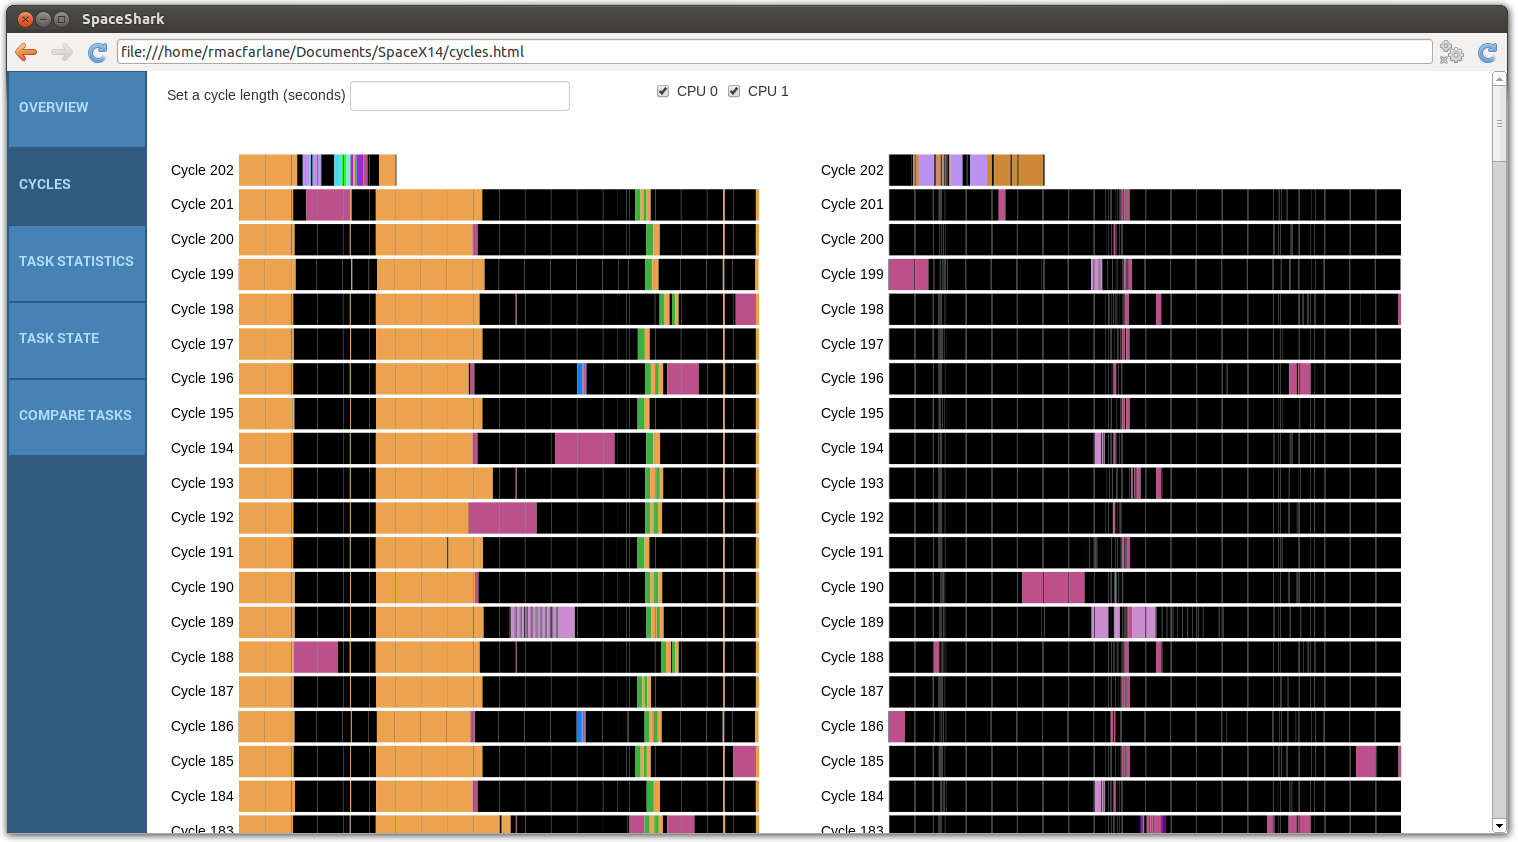
\includegraphics[scale=0.25]{cycles-page.png}
  
The idea behind the cycles page was to be able to find anomalies quickly. Having the main graph split up into cycles, can clearly show the user where something strange might be happening. More specifically, if there is a spot in the graph that doesn't show up in any of the previous cycles, then that point would be of particular interest to SpaceX engineers.

    The code for the cycles page is within assets/js/cyclesPage.js. This once again
    uses gantt-chart-d3.js to create the visualization after fetching the data.
    The page also has buttons to toggle on and off different CPUs, which removes
    or adds charts for these CPUs, rescaling other charts to use the full window
    space. Cycles are precomputed if print events exist within the trace. If
    not, the page will be blank when it first renders. The user can enter a
    number in the top box to set the period of desired cycles, which will then
    display a chart of cycles of that length. This feature also works even if
    print events are present in the data.
  
  \subsection{Task Statistics Page} %May Lynn

  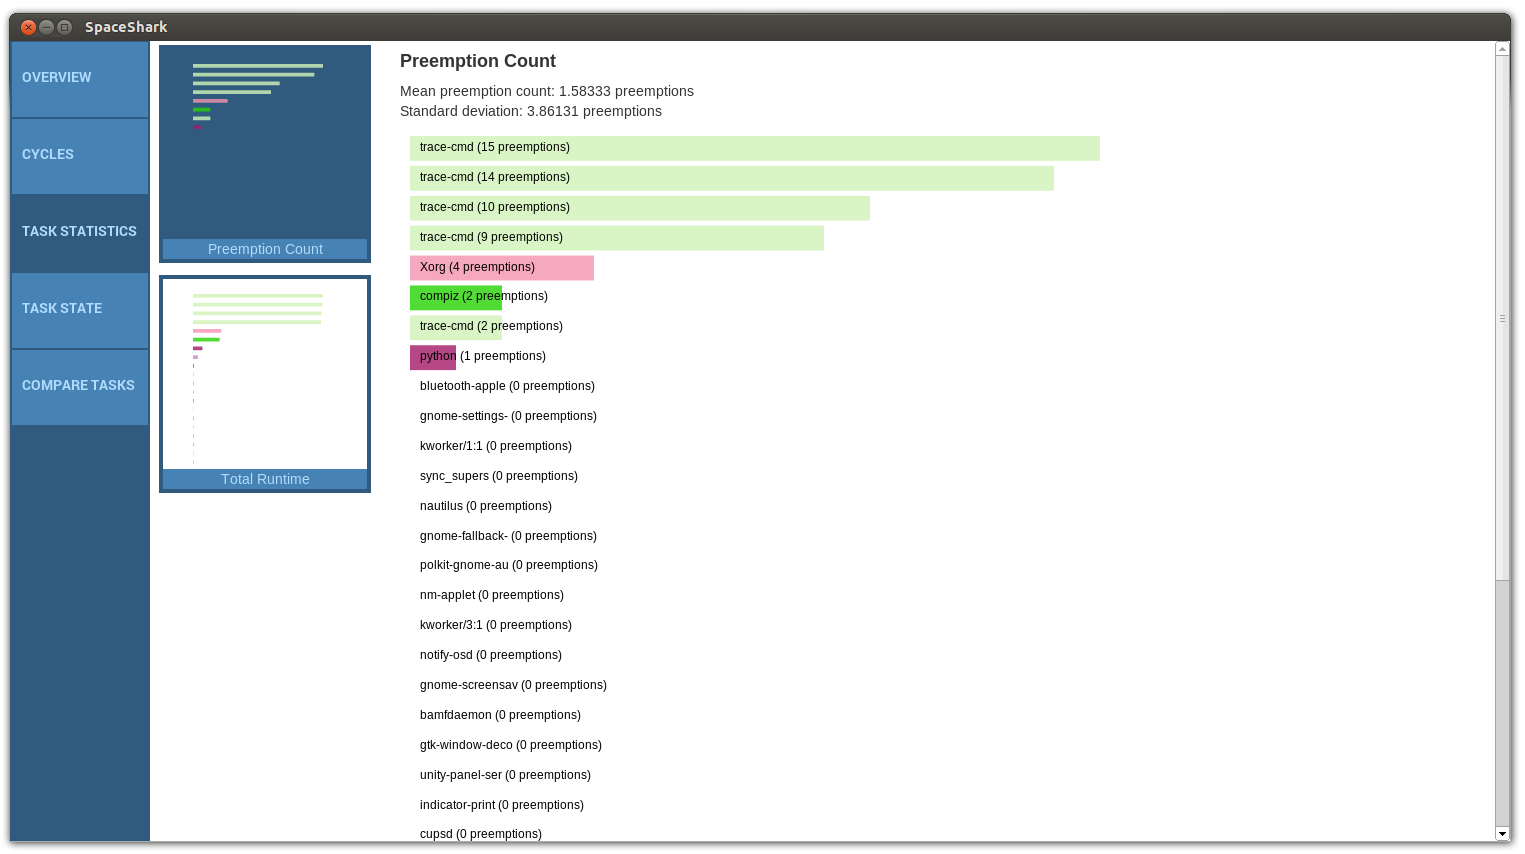
\includegraphics[scale=0.25]{task-statistics-page.png}

The purpose of the Task Statistics page is to give an overview of the preemption count and runtime of each task. The page displays bar charts of the preemption count and runtime for each task, sorted from highest to lowest, as well as the averages and standard deviations of each. This makes it very easy to see if there are any outliers with a large number of preemptions or a long runtime, or to check if a task is behaving as expected.

The code for this page is within assets/js/preemptionChart.js and assets/js/runtimeChart.js. The bar graphs use the dc.js dimensional charting library.

  \subsection{Task State}

  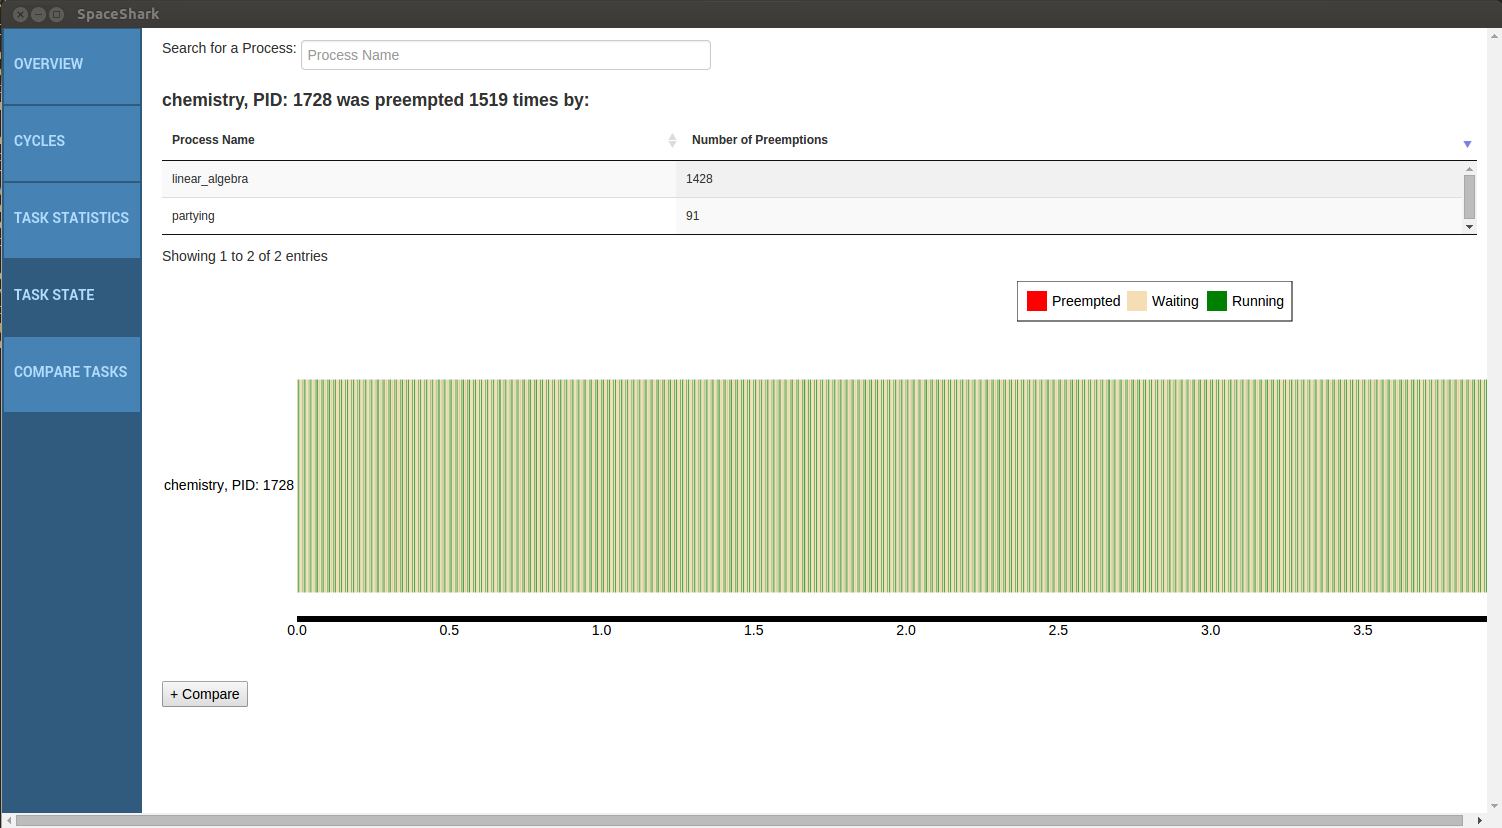
\includegraphics[scale=0.25]{task-state-page.png}
  
    The purpose of the Task State Page is to be able to look at a specific view of a
    process and potentially find something strange, such as a process being
    unexpectedly preempted many times. A table showing how many times the task was preempted, and by which task is shown, so that it is easy to spot if something is being unexpectedly preempted many times by a task that should not be preempting it. The graph of the task is color coded based on the current state of the task, so that the user can see at a glance when the task is running, waiting, or preempted, as well as how much time the task is spending in these states. This can make it easier to find potential priority inversions. The user can click the ``+ Compare'' button
    at the bottom to add this to a series of side-by-side graphs for comparison, which is described in the next section.

    The code for this page is within assets/js/process.js. This page uses
    gantt-chart-d3.js for the chart and dataScroller.js to create the table of
    preemptions. The search box autocompletes task names using twitter
    typeahead.
  
  \subsection{Compare Tasks} %Wendy

  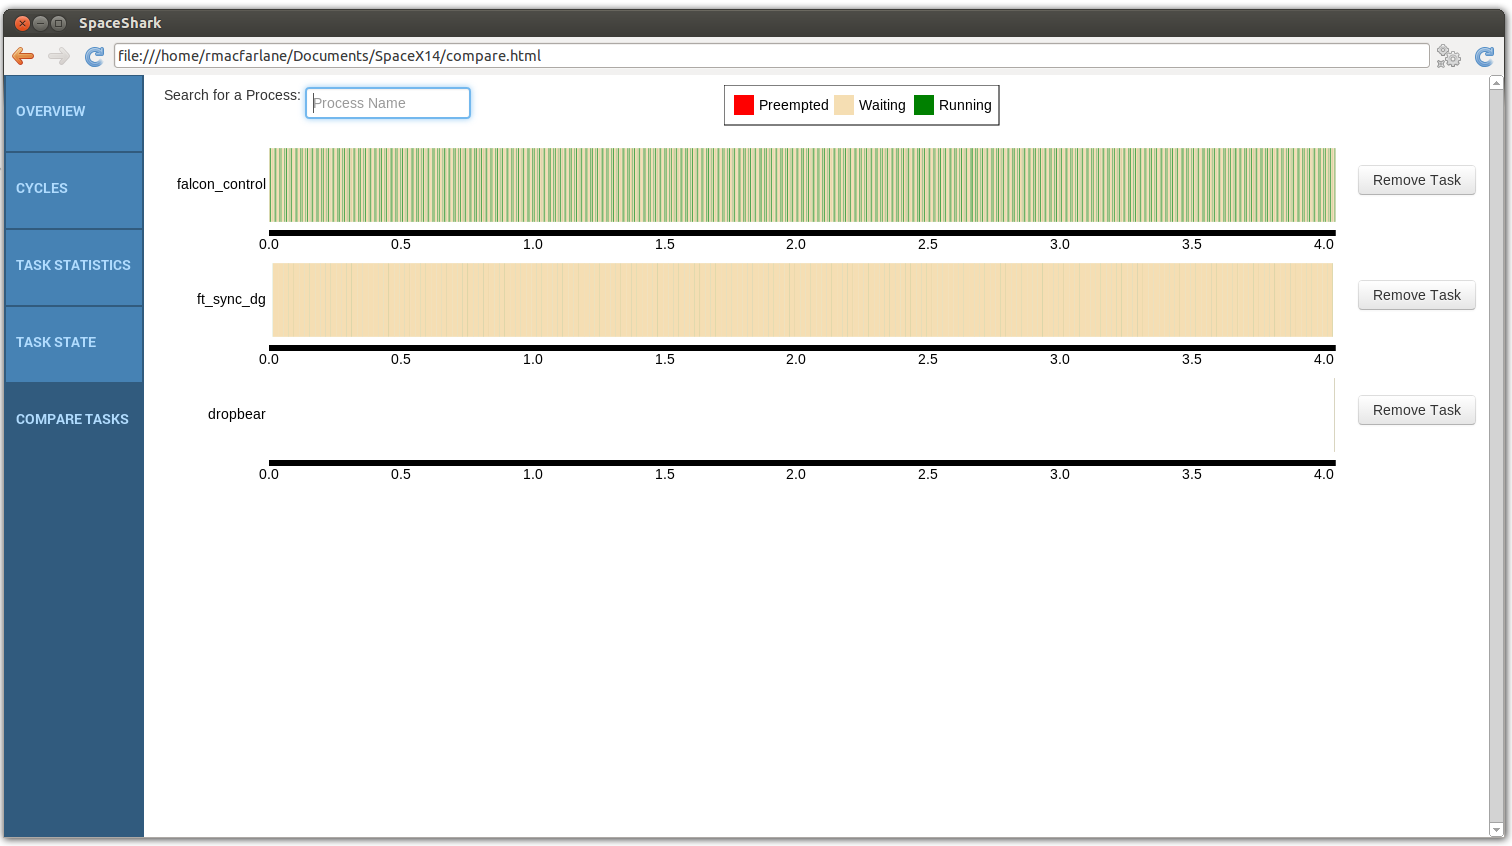
\includegraphics[scale=0.25]{compare-page.png}
 
The Compare Tasks page allows users to view the same graph as the Task State
page, but for multiple tasks. Tasks can be reordered so that specific tasks can
be compared side by side for the same time period. This provides similar
functionality as the Task State page but with the additional benefit of
comparisons between tasks. This makes it simple to examine interactions between two or more tasks, to see how they are affecting one another.

The code for this page is within assets/js/process.js. This page uses
    gantt-chart-d3.js for the chart, and draggabilly.js and packery.js to make the rows of graphs rearrangable.

\section{Architecture} % Wendy

  \subsection{Overview}
\begin{center}
  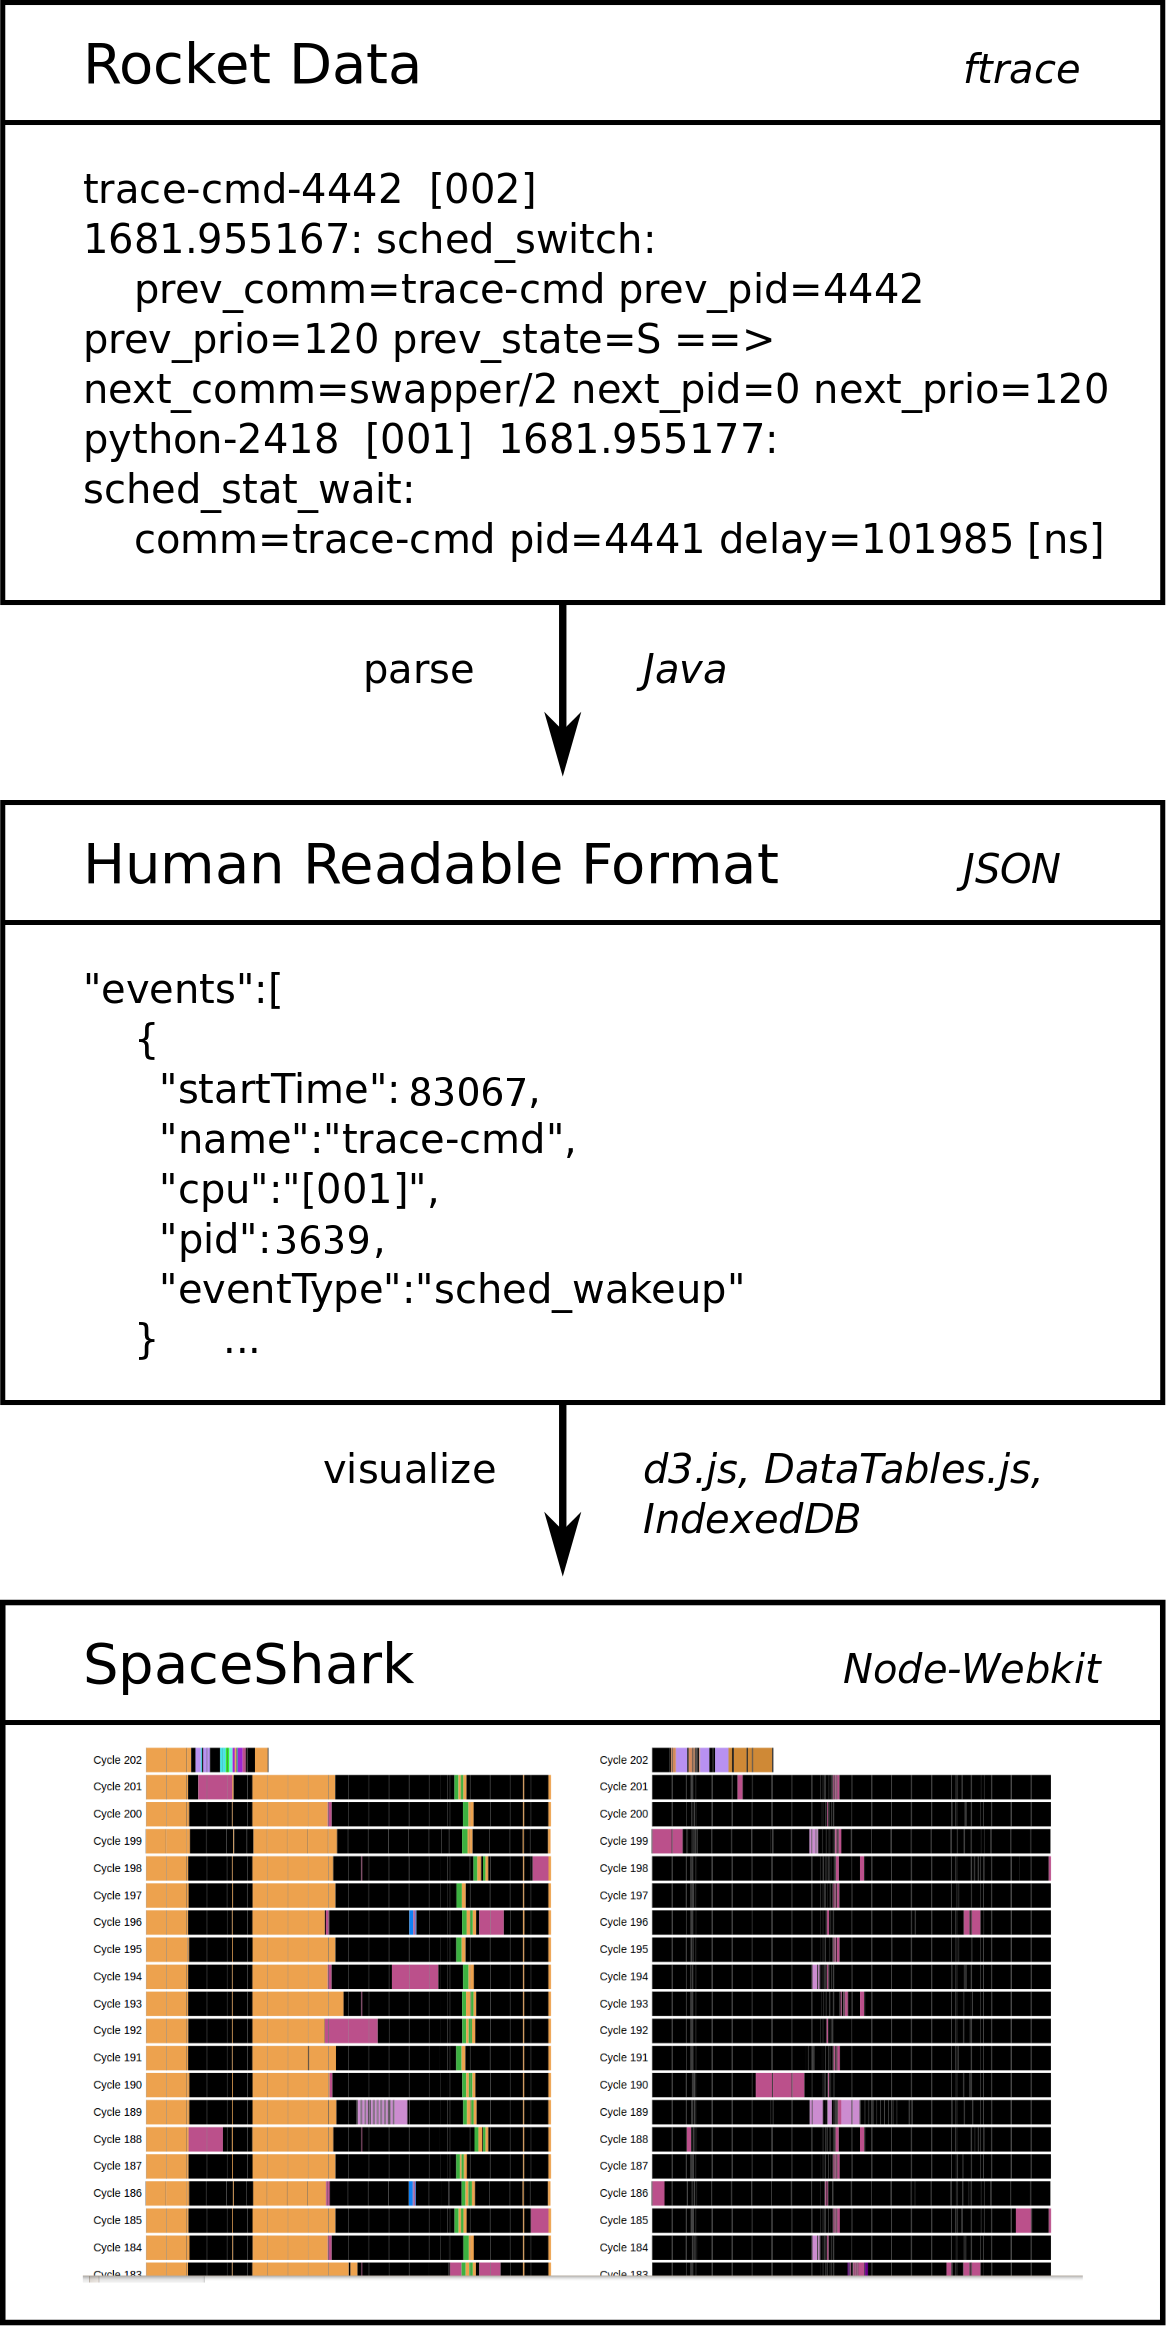
\includegraphics[scale=0.18]{architecture_diagram.png}
\end{center}
  Our application has three main portions: the raw input, the parser and it's
  output, and the web-based desktop application. The sections are modular, and
  as long as output/inputs remain the same, internal changes to one section will
  not affect the other at all.

  \subsection{Trace-cmd}

  Data is collected by using a command-line utility called trace-cmd.
  trace-cmd records various events in the Linux kernel while it runs and then
  outputs this information into a data file with a particular binary format.
  trace-cmd is a powerful tool and can be used to trace many different types of
  events. The type of events records are specified by the user when they run
  the tool. Our goal is to help visualize scheduling data: what tasks were
  scheduled to run, wait, and migrate between CPUs over the time of the trace.
  We therefore assume that the user has taken a trace that captures scheduling
  events.

  Besides outputting data in binary format, trace-cmd also has a ``report``
  option, which takes an existing trace file and generates a human readable
  report of this record. Using this format as a starting point instead of the
  raw binary format simplifies parsing.  We decided to leverage trace-cmd report
  instead of wrestling with the binary data ourselves. This allowed us to make
  progress faster and to avoid working on an already solved problem.

  The downside of this is that the format of the file generated by trace-cmd
  report is dependent on the version of trace-cmd used. To be able to reliably
  parse data and add additional information about preemptions, we need our input
  data to have a consistent format. This creates a dependency on a particular
  version of trace-cmd. Our liaisons have been using trace-cmd version 2.2.1, so
  our parser expects input data to be in the format of 2.2.1.

  \subsection{Parser}
  Next the parser takes in this raw data, and ultimately outputs the data
  reformatted into JSON with additional information. As a result of the
  particular version of trace-cmd, we know exactly how the file will be
  formatted. Each line in the input file is a single recorded event with a
  number of fields separated by whitespace. An example is shown below.
   
\footnotesize\begin{verbatim}<idle>-0   [002]  2296.990243: sched_wakeup: comm=nautilus pid=2390 prio=120\end{verbatim}
  
\normalsize
  Here, the task associated with the event is ``idle'' which has a PID of 0. The
  second field gives the CPU number, and the third the the start time, which
  is measured in milliseconds since kernel boot. The event type, which is 
  wakeup, migrate, or switch for schedule events, is given after this. The last
  field is extra information and varies in formatting based on the type of
  event. For the wakeup event, the name, PID, and priority of the task
  being woken up are displayed.

  To parse these event lines, we read our file line by line and break on
  whitespace. Then it is easy to extract fields one by one. To deal with the
  extra information field at the end, we case on event type. Switch events
  are the only types of events that contain extra information that we need.  The
  extra information field of switch events gives the name, PID, and priority of
  the task being switched in for the currently running task. Importantly, it
  also contains a flag that indicates if the task being switched out transitions
  to a runnable or sleeping state. If the task is switched out and into a
  sleeping state, it has been blocked, which means the event is a preemption.

  The parser also calculates the total runtime of each task by looking for
  ``sched\_stat\_runtime'' events. These events give the time elapsed between
  a task being switched in and out of a processor, so by summing them for 
  each event, we are able to add a field to a task giving total runtime.

  The output is formatted as a JSON file, so that we can easily transfer it to
  the web application. The JSON formatting has these elements:

  [see JSON format drive file]

  As long as this file remains the same, any changes to the internals of the
  parser will not affect the application itself. Additionally, this will allow
  someone with a different output to write their own parser to create the same
  type of output so that they can view their data in our tool.

  We were considering refactoring the parser to be cleaner. Currently, when we
  extract each field from an event, we immediately format it as a JSON object.
  This adds some additional complexity in later calculations and analysis, as
  the JSON object is a key-value pair, and is generally not very space or time
  efficient. Instead of this, it would be better to create an intermediate
  format for the data. We imagine this would look like a separate Java class for
  tasks and events. Events would be subclassed by their type. All events have
  the same basic information, like the start time, PID of the task involved, and
  CPU, but their extra information field varies based on type. We imagine that
  creating event and task classes would make the parser code much more readable,
  as after grabbing each field from a line, this information would be passed off
  and dealt with elsewhere. Given enough time, we would refactor the parser in
  this way, but as it is currently functional, these changes have not been high
  priority.

  The parser has not been packaged with the application, and currently stands as
  it's own tool.

  \subsection{Web Application}

  \subsubsection{IndexedDB}

  The application takes the JSON string and loads it into IndexedDB, a
  browser-based database. IndexedDB is built into most browsers, including
  node-webkit. More information on the details of IndexedDB can be found here
  (https://developer.mozilla.org/en-US/docs/Web/API/IndexedDB\_API).
  We use IndexedDB to store data between pages. It also
  maintains storage between application sessions. Therefore, we are able to have
  the choice to load the same file again, without reselecting it. If the user
  chooses to load a new file, we just write over this.
  Specifically, we store 
  \begin{itemize}
    \item numCPUs (number of CPUs for this file)
    \item cycleEvents (the events divided into cycles for the cycles page)
    \item Tasks (a list of all the tasks with various information)
    \item AutocompleteNames (used for autocomplete in search bars)
    \item AutocompleteEventTypes (also used for autocompleting)
    \item Events (a listing of all the events)
  \end{itemize}
  These correspond to the JSON types laid
  out in the Parser section (presumably we have numbers/pages later).

  Using the node-webkit profiling tool, we can see that IndexedDB is the slowest
  part of our application, as transactions with the database must be opened and
  closed. Ideally, we would use something less complex, but other options such
  as Local Storage did not have enough space for our large files.

  IndexedDB also has  a size limit, but this is typically not reached except for
  unusually long files or files with 4 or more CPUs.

  \subsubsection{Local Storage}

  Our application also makes use of Local Storage, another tool
  built into most browsers and node-webkit. This is a small and quick to access
  storage method. We primarily use it to save state between pages, notably
  display states. One example is the zoom level of the graph, which does not
  change between loads of the same page. Local Storage is also retained between
  application sessions. Similarly to our IndexedDB data, if the user chooses to
  load the same data we still have their state changes saved. If they load a new
  file Local Storage is cleared.

Here is a list of the Local Storage variables that we are using, and what they are for:
\begin{itemize}
\item cellData: A string containing the name and PID of the task currently being shown on the Task State page 
\item compareCurrScale
\item compareCurrTranslateX		
\item compareCurrTranslateY		
\item compareData: A list containing strings with the names and PIDs of the tasks currently being shown on the  Compare Tasks page
\item currScale	
\item currTranslate	
\item currTranslateX	
\item currTranslateY	
\item cyclesCurrScale	
\item cyclesCurrTranslateX		
\item cyclesCurrTranslateY		
\item displayedCPUs: A list of the CPU numbers that are being displayed on the Cycles page
\item firstEventTime	
\item hasEverExisted: We check this variable to see if there is content in Local Storage so that we know whether or not to give the user an option to use their previous data on the Load File page	
\item mainCurrScale	
\item mainCurrTranslateX	
\item mainCurrTranslateY
\item maxDuration
\item processCurrScale	
\item processCurrTranslateX		
\item processCurrTranslateY		
\end{itemize}
DataTables also makes use of Local Storage in order to save the scroll position of the table.

  \subsubsection{Overal Application Structure}

  The general structure of our code is similar to
  most web applications. In the root we have HTML files, which call to
  Javascript and CSS files, located in assets/js and assets/css respectively.
  HTML files do not have any Javascript or CSS inside them, but exclusively call
  to other functions for this. Each page has its own specific Javascript file,
  and then there are a number of shared files that multiple or all pages use. We
  have used a number of Javascript libraries.
  \subsubsection{Creating a Timeline}
  On the overview, cycles, task state, and task compare page, the same type of
  chart is used. The chart shows either which task is running at a given time,
  or what state a process is in at a given time. The chart is fed a list of
  events to display and a number of optional settings before being drawn. The
  array of all events needs to be passed through several helper functions
  before it is ready to be given to the graph.
  
  \begin{itemize}

    \item The events list is filtered to only contain switch events. Switch
      events are all that are needed to determine which task was running, or
      what state a task was in.
  
    \item All start times are normalized so that first event is at time zero.
      In the original events list, the start times of events are given in
      milliseconds since kernel boot, which is not relevant. We separate our
      events by CPU, and for each grouping of events, shift the start times
      so that the first one occurs at zero. (was this necessary to do?)
  
    \item The graph needs to know its time domain, so we calculate this
      endpoint. How this calculation is performed depends on which page we are
      on. On the overview page, we want to compare across CPUs. Each CPU may not
      be processing tasks for the entire duration of the trace. For example, all
      events on CPU 0 might take only 3 seconds, while all events on CPU 4 take
      4. We take the maximum of the total duration of events across CPUs, in our
      example, 4 seconds. The same calculation is used for the compare page so
      that the time range on the x-axis will be the same across all tasks.  On
      the cycles page, our time range is simply the length of a cycle.
  
    \item The gantt chart is passed its parameters in preparation to be drawn,
      not including the events. These parameters include the name of the page it
      is currently on, which will allow it to modify its behavior based on
      context, as well as what attribute to group by (CPU, cycle, or nothing).
      Width and height can also be passed, which allows charts on the compare
      page to take up little vertical space, while the overview page chart uses
      as much space is available to it.
  
   \item The events have their duration calculated, to determine how large each
     rectangle should be drawn. For example, on the main page we calculate the
     difference between the start times of consecutive switch events. This gives
     us the amount of time each task was running for.
  
   \item The gantt chart is passed the events and drawn, and the colors are set.
     The chart assigns a class to each task based on its PID, and we randomly
     select a color for this class and add a style tag to the page. Our random
     color selecton is seeded so that the same colors will be assigned every
     time. We considered producing a stylesheet after parsing so we did not have
     to generate this each time, but in profiling the application we saw that
     this process was actually quick, and decided this change was very low
     priority.

  \end{itemize}
  \subsubsection{Primary Javascript/CSS files}
  One of the primary Javascript files we've worked
  with and changed is gantt-chart-d3.js. This file is the logic for all of the
  graphs. This file was originally written by Dimitry Kudrayvtsev, but we have
  significantly modified it to produce the behavior we want. The file begins
  with global variables and definitions for default settings. From lines
  115-195, we define zoom behavior. aaaah wendy explain how zooming works.
  226-325 actually render the graph, adds hovertext and other attributes. The
  last portion of the code makes it possible for the user to set different
  parameters of the graph when it is created.

  Sidebar.js is a fairly simple script that creates the sidebar for all of the
  pages, excluding the first page of the app, where the user chooses a file.

  The other non-page specific files are mostly borrowed and unedited from
  Javascript libraries, so for documentation on those you can visit their
  respective pages online.
\begin{itemize}
\item d3.js (d3js.org)
% d3 - http://d3js.org/
\item dc.js (dc-js.github.io/dc.js)
% dc - http://dc-js.github.io/dc.js/
\item Draggabilly (draggabilly.desandro.com)
% draggabilly - http://draggabilly.desandro.com/
\item Packery (packery.metafizzy.co)
% packery - http://packery.metafizzy.co/
\item DataTables (datatables.net)
% datatables - https://www.datatables.net/
\item Twitter Typeahead (twitter.github.io/typeahead.js)
% typeahead - https://twitter.github.io/typeahead.js/
\item Underscore (underscorejs.org)
%% FIXME - any more?
\end{itemize}

\chapter{User Feedback} % Alix
\section{General Feedback} % Alix
During a week long site visit at SpaceX, we were able to user test with four SpaceX engineers. 
User testing played a major component in making sure that we were creating a
tool that the engineers would be able to use to find errors in their rocket
software. We found a few discrepancies between what we thought would be useful
for engineers and what engineers actually found useful. Additionally, we were
able to see which aspects of the tool had been done well and gain a better
understand of how these features helped SpaceX engineers. Overall, user testing
provided a good way to ground our project, by showing us what worked and what
didn't, so that we could really be sure our tool was useful and make decisions
accordingly. We will focus mostly on the negative feedback, as critical feedback
was the most useful in moving forward to improve the tool.

A common theme was that our tool was not cohesive. There wasn't enough
connection between the different sets of data our tool used. Context is really
important to SpaceX engineers. The way a task behaves by itself isn't really
enough to understand what is going on with the computer as a whole. Seeing the
interactions of the entire system is more useful than individual pieces.

\section{Methodology} % Wendy
In order to test our tool, two members of our team would watch an individual
work their way through it using our sample data, or in some cases the user's
data if they had some prepared. We tried to provide as little
input as possible, except for encouraging the team member to think out loud and
talk about what they were thinking, expecting, or doing, and why. While the user
did this, we would take notes on both what they were saying and what they were
doing.

Once the user felt like they had explored the tool, we talked more in-depth
about their experience, also elaborating on our intent with the tool,
encouraging explicit feedback on how we could make the tool better. A large
portion of this process went to brainstorming with the user and finding out why
a page was helpful or unhelpful for their specific workflow.

\section{Feedback on Specific Pages} % Alix

\subsubsection{Main Page}

The main page of KernelShark featured a graphical display of the processes
running over time and a tabular version of the same information. KernelShark had
a number of problems, including poor user interface, unintuitive zooming,
features that did not work as expected, and a limited way to view the data.
Using KernelShark required the user to know the behavior they expected to see
beforehand, as it did not provide any indication of cycles or features aimed
specifically at detecting errors.

Before winter break, our tool featured a graphical representation of tasks running over time,
as well three tables that displayed the top ten preempted, longest running, and
longest waiting tasks. 
Through user testing, we found that three out of four users mentioned that they
did not find the statistics on the Overview page helpful. Because only one user found the statistics useful,
we decided as a team that it would be best to omit them from the Overview page, and
only display them on the Task Statistics page.

Additionally, the Overview page initially only showed the graphical
representation. Two of the users mentioned that the typical workflow of the tool
would be to visually find the problem in the graph, zoom in to that particular
strange spot in the graph, be able to jump to that spot in the events list, and
then scan a tabular version of the events list. In order to have this workflow,
we would need to have the tabular version of the graph on the Overview page.
As a result we decided that the Overview page of our tool would have both the
graphical version of the time series data, as well as the tabular version of it.
This gives our Overview page the context that SpaceX engineers are looking for.
It is easy to find something interesting on the graph, and then get the details
on it via the tabular display.

This figure shows what our Overview page currently looks like:
\begin{center}
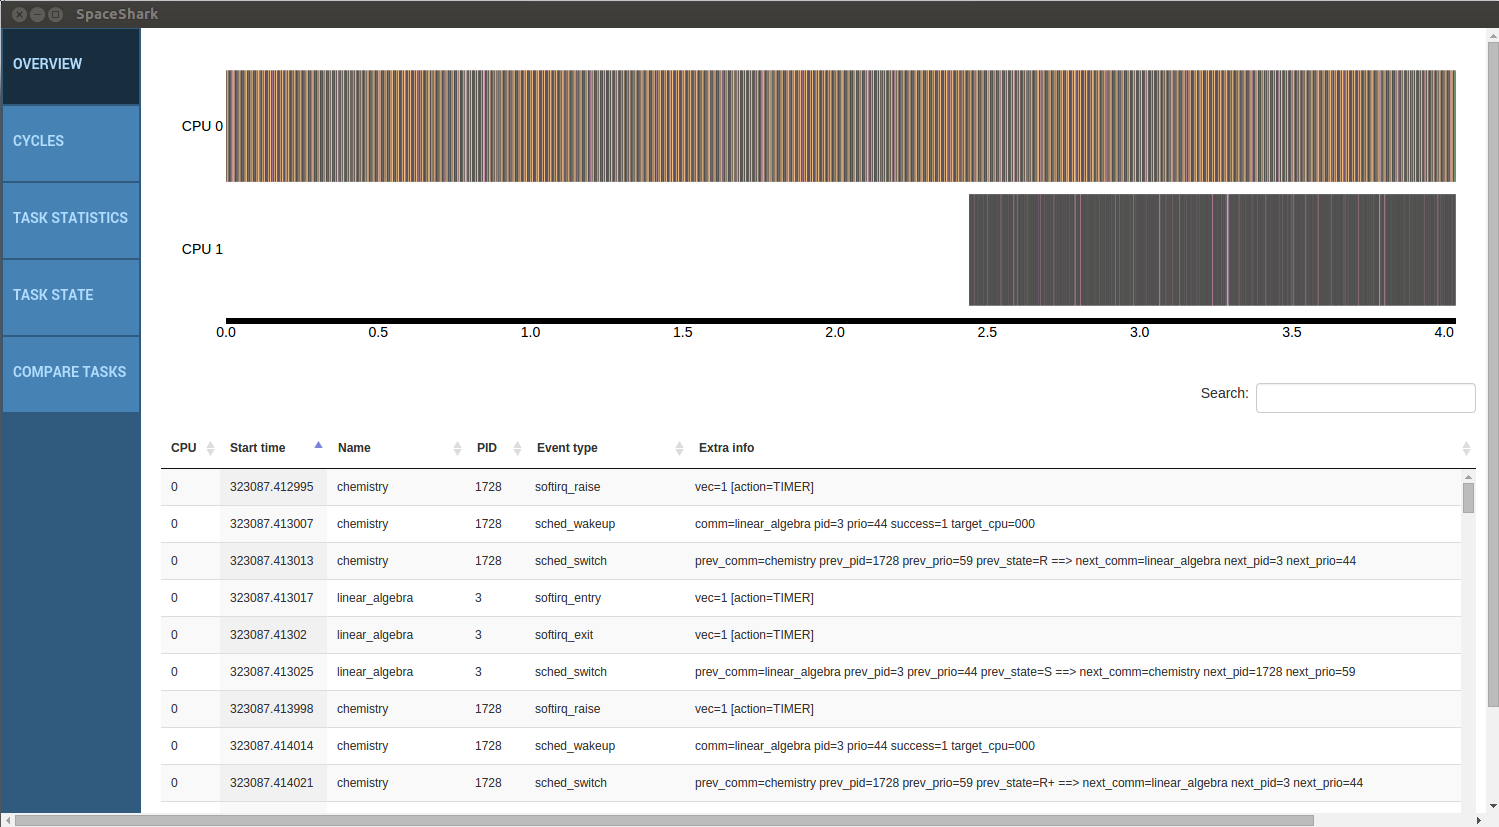
\includegraphics[width=4in]{overview-page.png}
\end{center}

Our Overview page mimics a lot of the good
functionality that KernelShark had. Additionally, it allows users to filter the
tabular list of events on a variety of properties, and jump directly from a
specific point in the graph to the same point represented in the table. Double
clicking on a particular task in the table will also take the user to the
Process page, where they can get more information on a specific task. Covering
much of KernelShark's functionality on this page allowed us to use the rest of
our tool to surpass KernelShark's functionality and create a more versatile
tool.

\subsubsection{Task State Page}

With KernelShark, the user could pull out a graphical display of a single
task and put it on it's own line. However, that was the extent of what
Kernelshark did with regards to individual tasks.

We wanted to take this idea further by providing detailed information and
statistics about individual tasks. This would give users a different way to view
their data, hopefully expediting the debugging process.

\begin{center}
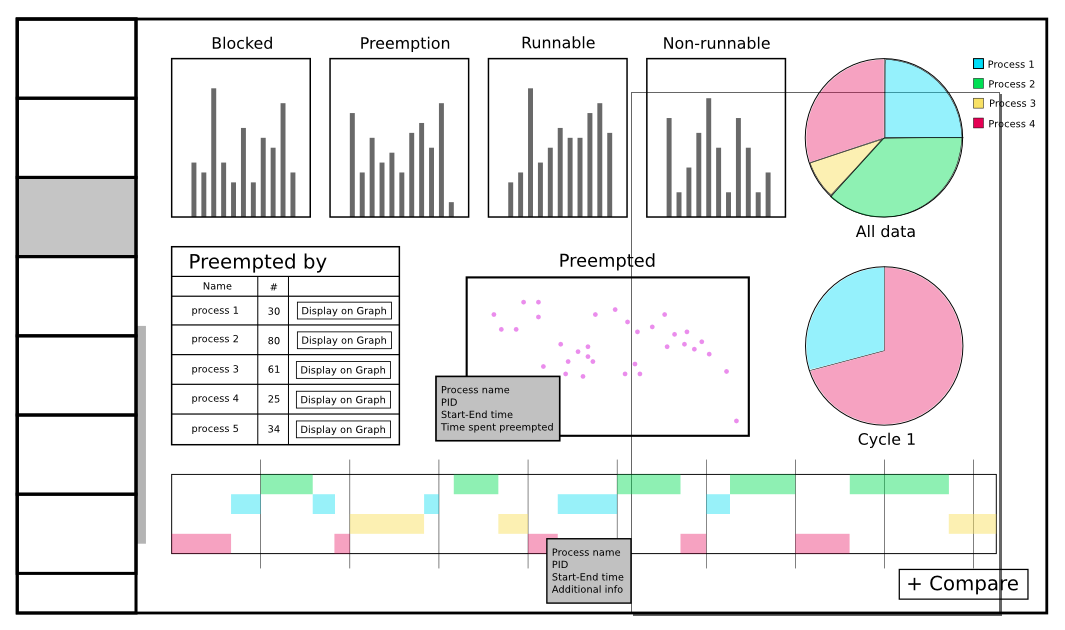
\includegraphics[width=4in]{perProcess-49.png}
\end{center}

Since there was no existing Task State page, we designed a mockup of it at the
beginning of the project. It features many different kinds of visualizations,
such as histograms of how long the task was in each state for, a scatterplot of 
what preempted it, a table of what preempted it, pie charts representing the 
data in cycles, and a graphical display of the time series data highlighting 
the process in the graph. Through user feedback with the liaisons, we found 
that our mockup included way too much information that SpaceX engineers would 
not have found useful. Since preemptions are of most interest and are generally
the indicative of problems, we really wanted to focus on this on the Task State
page.

\begin{center}
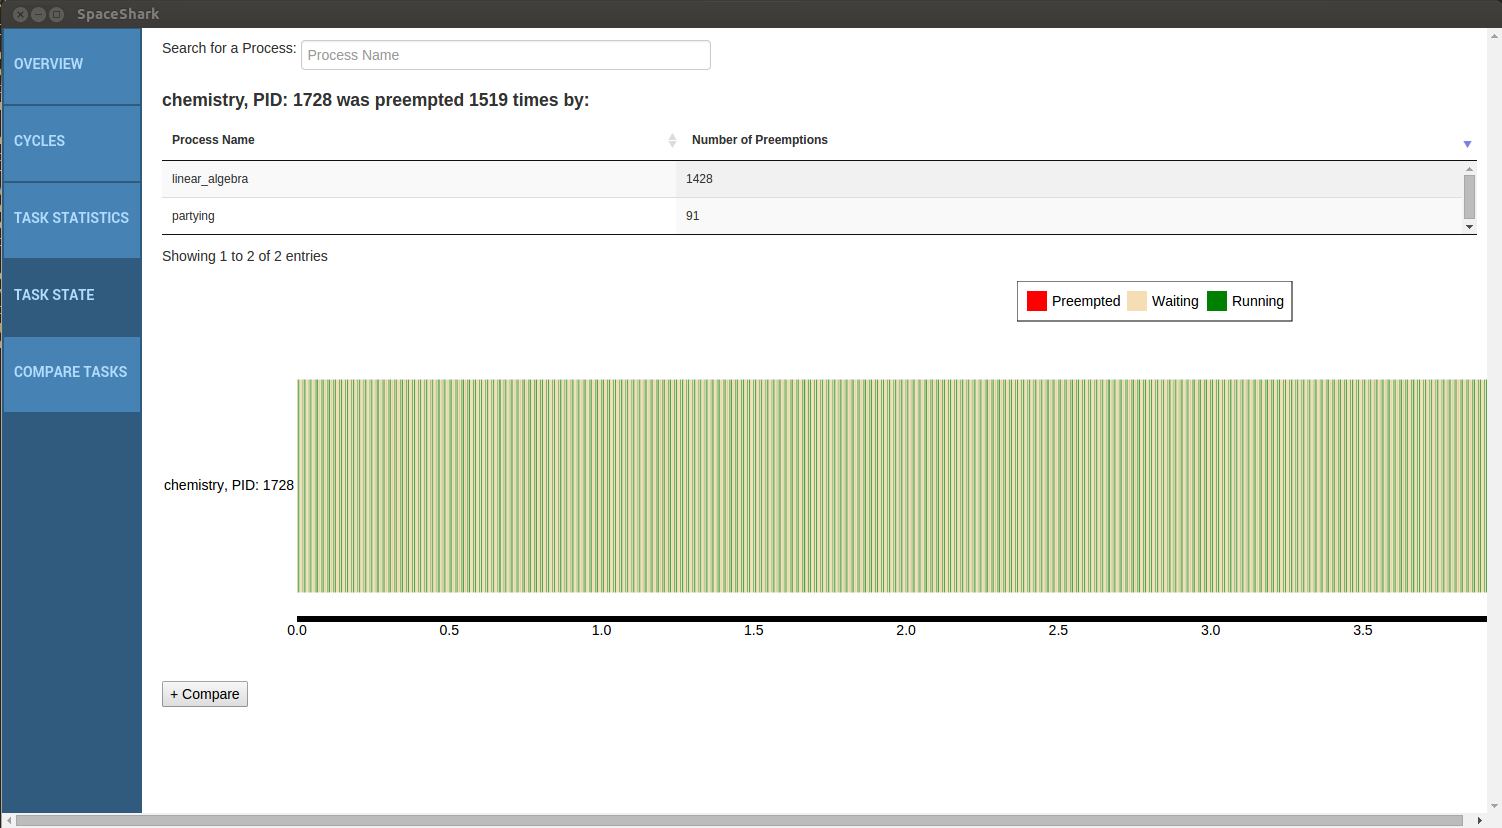
\includegraphics[width=4in]{task-state-page.png}
\end{center}

On the Task State page, the user is able to type in a particular process, see
how many times it was preempted and which processes preempted it, as well as
view a graph showing how long it was in one of three states: running, waiting,
or preempted. This design has a minimalistic page view compared to the mockup,
but makes better use of the information it provides, and includes less
extraneous, unhelpful information.

This pages allows SpaceX engineers to find information on specific tasks, which
is something that KernelShark was unable to do. It helps engineers dig in to the
details, especially when used in conjunction with the broader context provided
on the Overview page and other pages.

When user testing, we received feedback that this page needed more context,
prompting us to create the Compare Tasks page. The Compare Tasks page has not
yet been user tested, but we hope it will meet this need by allowing users to
display multiple state graphs side by side to look at anomalies in context.

\subsubsection{Cycles Page}

One of the most notable things that separates our tool from KernelShark is that
KernelShark did not provide information about cycles, meaning that users had to
manually determine where cycles were.
The Cycles page in our tool lets the user easily find anomalies by splitting up
the Overview page graph visualization into cycles.

The following image shows our initial mockup of the Cycles page:

\begin{center}
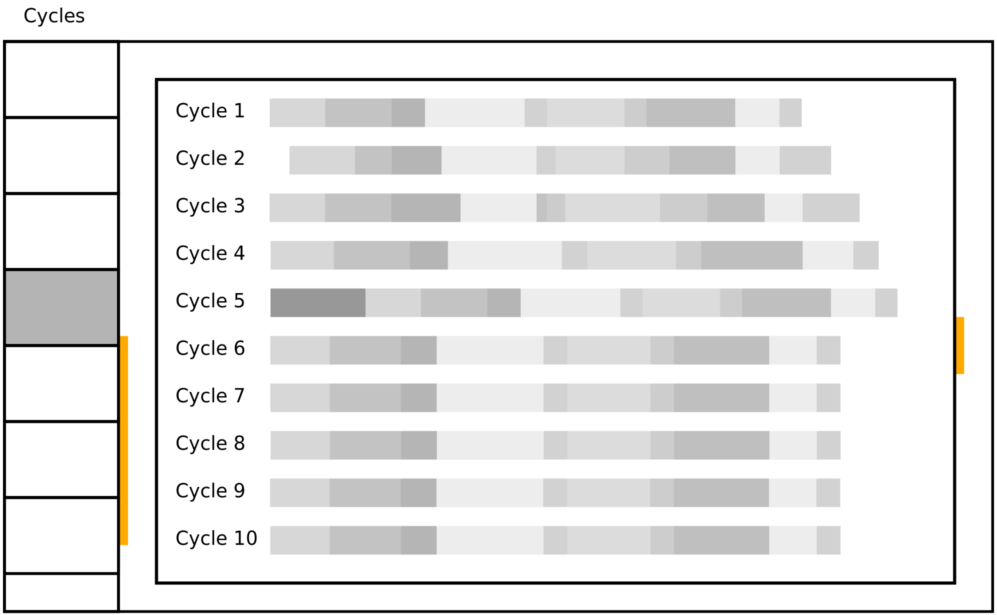
\includegraphics[width=4in]{oldcycles.png}
\end{center}

We received nearly all positive feedback on the Cycles page, and this seems to
be the most useful aspect of our tool.

The first change  we made was very minor; rather than ordering the cycles from first cycle to last cycle, we changed it to be ordered from last cycle to first. We made this change because anomalies are normally found within the last cycle, which SpaceX engineers would want to see displayed prominently at the top of the page.

Additionally, this page initially relied on the user's code generating ``cycle
markers'', which meant that this functionality would not have worked with old
traces, or traces that didn't conform to our specific markers. One engineer
suggested that we add the ability to enter in cycle length and have it display
cycles based on that. We chose to implement this, taking this page from having
very specific requirements to being usable with any data.

\chapter{Challenges}
\section{trace-cmd versioning} % Rachel
  As already described, we collect data using a command-line utility called
  trace-cmd. trace-cmd records various events in the Linux kernel while it runs
  and then outputs this information into a data file with a particular binary
  format. trace-cmd also has a ``report'' option, which takes an existing trace
  file and generates a human readable report of this record. Using this format
  as a starting point instead of the raw binary format simplifies parsing.
  We decided to leverage trace-cmd report instead of wrestling with the binary
  data ourselves. This allowed us to make progress faster and to avoid working
  on an already solved problem.

  Unfortunately, the format of the file generated by trace-cmd report is
  dependent on the version of trace-cmd used. For example, the formatting of the
  ``extra info'' field of a switch event is liable to change. We use this
  field to identify preemptions. To be able to reliably parse data and add
  additional information about preemptions, we need our input data to have
  a consistent format. This creates a dependency on a particular version
  of trace-cmd. Our liaisons have been using trace-cmd version 2.2.1, so
  our parser expects input data to be in the format of 2.2.1.
\section{Selection of charting tool} % Rachel
  We chose to use web technologies because we felt there was a wealth of
  charting and UI/UX tools that we could use. We spent several weeks
  experimenting with different charts for the main page. The main page renders a
  timeline of running tasks, which is essentially a large number of colored
  bars. This chart needed to be responsive to zooming and dragging, and to
  dealing with click events to move to a particular time in the table of events
  displayed below it.
\section{Speed} %Wendy
The data SpaceX will be using with our tool is very large, and becomes even
larger once we have parsed it. As a result, some parts of the tool load slowly,
and this is something we are still working on fixing. One main fix we have
implemented is batch loading the list of events on the main page so that the
user can start interacting with the tool without waiting to load the entire
table, especially since all of the table is typically not needed.

Having done some profiling, we know that pulling data from IndexedDB is the
slowest part of our application, but at this point in time we do not have a way
to fix this.

\chapter{Future Work}
\section{Known bugs}
  
All graphs can be dragged until they become no longer visible. While they can
be dragged back using the white space, this is not good for a user experience.

Graphs and other images do not resize when the window resizes unless the page
is reloaded.

Zooming in on a graph removes the graph name. Additionally, the x-axes do not
develop more ticks as you zoom in, making it harder to get a sense of scale.

\section{Extensions}
  SpaceX developers indicated an interest in interleaving the graphs of multiple
  CPUs on the Cycles page.  This would make it easier to compare cycle
  anomalies across CPUs, as this would cause the timestamps to align. Making
  this possible would require tweaking the graph infrastructure, and creating an
  interface for users to choose if they want the graphs interleaved or not, and
  which cycle numbers to display.
\section{Scalability}
  Overall, the application should be made faster. We are not entirely sure how
  to improve this at the moment. IndexedDB is the slowest part of the
  application at current.

Additionally, if given files above a certain size, typically using more than 4
cores, the parsed version will be too large for IndexedDB to load, and
sometimes too large for the parser to handle as well.

There are two possibilities for fixing this. One is to prune the JSON or
finder a more compressed method of storing the data. The other is to find a
substitute for IndexedDB that is faster.
\section{more user testing - results}

\end{document}



